
\section{Caraway}
\label{sec:caraway}

\begin{spice}\label{spice:caraway}
\textsc{Caraway} \hfill \href{https://powo.science.kew.org/taxon/839677-1}{POWO} \\
\textbf{English:} \textit{caraway}. 
\textbf{Arabic:} {\arabicfont{كراويا}} \textit{karāwiyā}. 
\textbf{Chinese:} {\tradchinesefont{葛縷子}} \textit{gě​lǚ​zi}. 
\textbf{Hungarian:} \textit{fűszerkömény } [spice-cumin].  \\
\noindent{\color{black}\rule[0.5ex]{\linewidth}{.5pt}}
\begin{tabular}{@{}p{0.25\linewidth}@{}p{0.75\linewidth}@{}}
Plant species: & \taxonn{Carum carvi}{L.} \\
Family: & \textit{Apiaceae/Umbelliferae} \\
Plant part used: & fruit \\
Region of origin: & Mediterranean; Eurasia \\
Cultivated in: & Denmark, Lebanon, The Netherlands, Poland \\
Color: & nan \\
\end{tabular}
\end{spice}

% \begin{figure}[!ht]
% 	\vspace{-4ex}
% 	\centering
% 	\subfloat[\centering a]{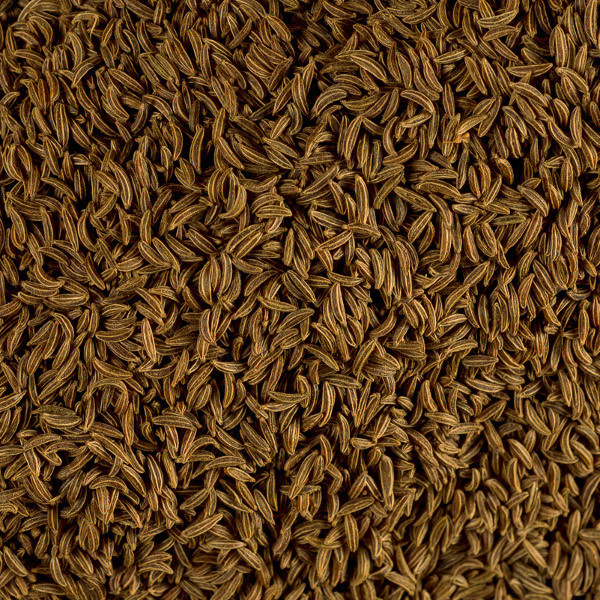
\includegraphics[width=0.3\linewidth]{imgs/spices/caraway-1.jpg}}
% 	\hfill
% 	\subfloat[\centering b]{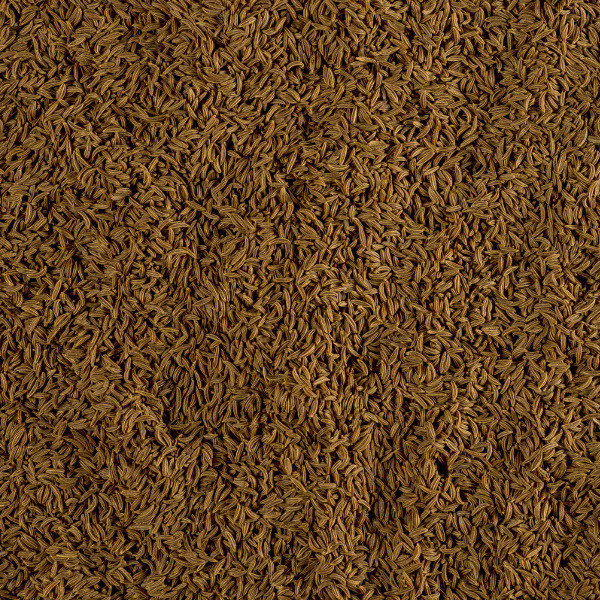
\includegraphics[width=0.3\linewidth]{imgs/spices/caraway-2.jpg}}
% % 	\hfill
% % 	\subfloat[\centering c]{\includegraphics[width=0.3\linewidth]{imgs/spices/caraway3.jpg}}
% 	\caption{Caraway \textit{Carum carvi}.}
% 	\label{fig:caraway_imgs}
% \end{figure}

\begin{wrapfigure}{R}{0.33\textwidth}
	\vspace{-\baselineskip}
	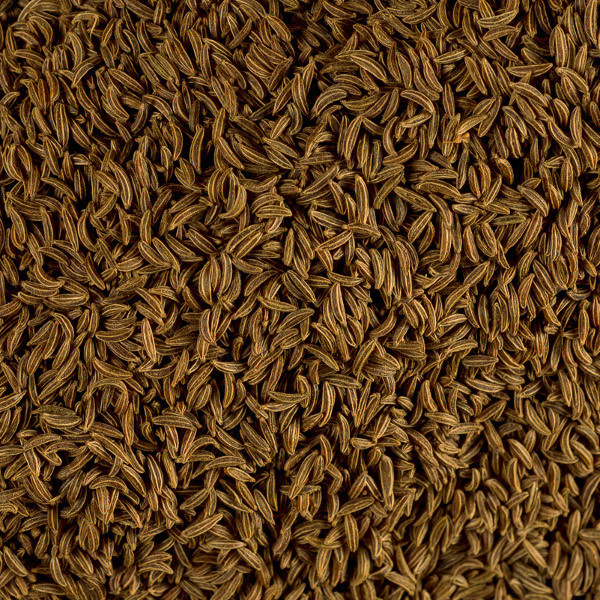
\includegraphics[width=0.33\textwidth]{imgs/spices/caraway-1.jpg}
	\caption{Caraway-seeds (fruits, \textit{Carum carvi}).}
	\label{fig:caraway}
\end{wrapfigure}

Caraway-seeds are in fact the fruits of the plant \textit{Carum carvi}, and they are longer, narrower, and darker than cumin (\textit{Cuminum cyminum}). The two are often confused, both in language and in the kitchen. Caraway hs a visible ``rib'' along the curve that makes the two mericaps (two halves of a compact fruit) better observable \autocite[100]{van_wyk_culinary_2014}. Caraway has a somewhat peppery and bitter, but mild aroma that makes it a popular choice of spice on the vast regions it grows. 

As a spice, caraway is popular in European cuisines, it is used to flavor bread, cheese, sausages, soups, the famous German \textit{sauerkraut} and even alcoholic beverages \autocite{van_wyk_culinary_2014}.

% Caraway has often been confused with the similar-looking cumin, as can be seen in vernacular names that originally referred to cumin (derived from the Latin Cuminum), such as Kümmel (German). Similarly, the Hindi name jeera is sometimes used for caraway but actually refers to cumin and black cumin (see Cuminum cyminum). 



% culinary uses Caraway is a typical spice of German-speaking countries and is an important flavour ingredient of rye bread, sauerkraut, Schweinsbraten (roast pork), goulashes, vegetables, potatoes, cheeses (e.g.,Munster), cakes and biscuits as well as alcoholic beverages such as kümmel, schnapps and vespétro.4 In the Netherlands, it is an ingredient of Leyden cheese, the most common type of kominjekaas. It is also a popular spice in Scandinavia, used to flavour food, confectionery, cheeses (e.g.,Swedish bondost and Danish harvati) and beverages (akvavit). In France, caraway is used to flavour dragées (sugarcoated almonds).4 In Britain it is often included in pickles and cabbage and traditionally served as a condiment (in a small dish) along with baked apples.2 It is popular in confectionery (e.g.,British caraway seedcake and Serbian scones) and desserts (e.g.,Middle Eastern caraway pudding). Flavour compounDs The warm, aromatic flavour of caraway fruits is due to essential oil rich in R-(+)-carvone (60\%) and limonene (40\%)5. S-(–) carvone smells like spearmint and is the main compound of spearmint oil (see Mentha spicata). Only the R-enantiomer of limonene occurs in nature. notes The fruits and essential oil are used to alleviate flatulence and stomach complaints.

% 1. Mabberley, D.J. 2008. Mabberley’s plant-book (3rd ed.). Cambridge University Press, Cambridge. 2. Kiple, K.F., Ornelas, K.C. (Eds). 2000. The Cambridge world history of food. Cambridge University Press, Cambridge. 3. Farrel, K.T. 1999. Spices, condiments and seasonings. Aspen Publishers, Gaithersburg, USA. 4. Larousse. 1999. The concise Larousse gastronomique. Hamlyn, London. 5. Harborne, J.B., Baxter, H. 2001. Chemical dictionary of economic plants. Wiley, New York.

\subsection{The Botany, Origin, and  Cultivation of Caraway}

Similarly to other spice plants in the umbelliferous family, the caraway plant is a small biennial herb with soft stems and umbels of small white flowers that bear the fruits people call seeds \autocite[100]{van_wyk_culinary_2014}. Caraway is indigenous in large areas of Eurasia: central Europe, the Mediterranean region, western and central Asia \autocite{mabberley_mabberleys_2017}. 
% The Romans used the roots as a vegetable. Caraway is now a popular spice in many parts of the world. 
Caraway is widely cultivated in Eastern Europe and German speaking areas, as north as Finland, but the bulk of caraway nowadays comes from Egypt \autocite{farrell_spices_1985}. The plants are grown from seeds, harvesting happens in the second year when the fruits ripen and turn brown \autocite{van_wyk_culinary_2014}.

\subsection{The History of Caraway}

Caraway is an ancient spice as indicated by neolithic samples, and according to \textcite[436]{kiple_cambridge_2000} it was always popular as a local alternative to expensive exotic spices.

\subsection{The Names of Caraway}

\subsubsection{English}

\begin{etymology}\label{ety:caraway}
English \textit{caraway}
< Medieval Latin \textit{carui} `id.', or some allied Romanic form; cf. cognates French carvi, Italian carvi, Spanish carvi (whence Scots carvy, kervie), Old Spanish alcaravea, alcarahueya, Portuguese alcaravia, alcorovia
< Arabic \textit{karawiyā} `id.', (loaned to some Eurropean languages with \textit{al-} definite article; via Andalusian Arabic)
< Aramaic {\he{כַרְוָיָא‎}/\sy{ܟܲܪܘܵܝܵܐ}} \textit{karwāyā} `id.'
< Ancient Greek {καρώ} \textit{karṓ} `id.', a form of the word \textit{káron}, derived from \textit{káre} `head'; -ṓ form seems Pre-Greek (these forms could not immediately give the Arabic, hence possibly via *καρυΐα \textit{*karuḯa} a typical plant derivation form of καρώ \textit{karṓ}, κάρον \textit{káron}); cf. cognates Latin \textit{carum, careum}\footnote{\textcite[s.v. caraway]{oed}; \textcite[s.v. caraway]{ahd}; \textcite[74]{corriente_dictionary_2008}; \textcites[207]{low_aramaeische_1881}[437-438]{low_flora_1924}; \textcites[653]{beekes_etymological_2010}[599]{sokoloff_dictionary_2002}}
\end{etymology}

English \textit{caraway} comes from a Romance language, such as  French \textit{carvi} (attested in 1256)\footcite[carvi]{tlfi} or the equivalent Medieval Latin \textit{carui} (ca. 1080), whence the scientific name.\footcites[caraway]{oed}[carvi]{tlfi} The Romance languages borrowed this word from Arabic \ar{كراويا} \textit{karāwiyā}, sometimes with the definite article \textit{al-}.\footcite{corriente_dictionary_2008} (Many Arabic loanwords in Spanish contain the definite article, and many of these borrowings go back to the times of Muslim Spain in al-Andalus, otherwise know as \textit{La Convivencia}; e.g., \textit{almohada} `pillow', \textit{alcatraz} `cormoran', \textit{alcohol} `alcohol', \textit{álgebra} `algebra', etc.)

The Arabic term has Semitic cognates in Aramaic, which is thought to be a loanword from Ancient Greek \gr{καρώ} \textit{karṓ}, (also etymon of \textit{carrot}), which shows sign of being pre-Greek.\footcite{beekes_etymological_2010}. According to \textcite{sokoloff_dictionary_2002}, the development of the Greek word follows typical plant name derivation patterns. The spice ajowan/ajwain \textit{Trachyspermum ammi} also has a synonym from this etymon: \textit{carom}.

Further English vernacular names use \textit{cumin} as the prototype word, and modify it with distinguishing words that Indicate the general direction and places where caraway was arriving from: the mountainous regions of Armenia and Persia. \textit{Royal cumin}---attested in 1614---seems to be a semantic translation of Hindustani \sa{शाह जीरा}/\fa{شاه جيرا} \textit{shāhjīrā}, a Persianate term that is modeled from the Farsi words \textit{shāh}
`king' (origin of the word \textit{check} in the ``checkmate'' of chess) and \textit{jīrā} `cumin', but its use is restricted to South Asia and not Iran. However, in the first record of it in ``A \lgS hort Table expounding all the hard words in this book'', it refers to bishop's weed, bullwort, or \textit{ammi} (ameos) (\textit{Ammi majus}), which another umbelliferous herb with similar seeds \autocite[]{markham_cheap_1614}.

\begin{table}[!ht]
\centering
\begin{tabularx}{\textwidth}{@{}l>{\itshape \small}lL>{\small}l@{}}
\toprule
\textbf{\#} & \multicolumn{1}{l}{\textbf{Species}} & \multicolumn{1}{l}{\textbf{Name}} & \multicolumn{1}{l}{\textbf{Source}} \\
\midrule
1	& Carum carvi	& Armenian cumin	& \textcite{oed} \\
\textbf{2}	& \textbf{Carum carvi}	& \textbf{caraway}	& \textbf{\textcite{van_wyk_culinary_2014}} \\
3	& Carum carvi	& caraway-seed	& \textcite{oed} \\
4	& Carum carvi	& meredian fennel	& \textcite{wikipedia} \\
5	& Carum carvi	& mountain cumin	& \textcite{oed} \\
6	& Carum carvi	& Persian cumin	& \textcite{wikipedia} \\
7	& Carum carvi	& royal cumin	& \textcite{oed} \\
\bottomrule
\end{tabularx}
\caption{Various names for caraway in English.}
\label{table:names_caraway_en}
\end{table}



\subsubsection{Arabic}

% \begin{etymology}\label{ety:karawiya}
\textbf{Arabic} \textit{karawiyā} `caraway', (loaned to some Eurropean languages with \textit{al-} definite article; via Andalusian Arabic)
< \textbf{Aramaic} {\he{כַרְוָיָא}/\sy{ܟܲܪܘܵܝܵܐ}} \textit{karwāyā} `caraway'
< \textbf{Ancient Greek} {καρώ} \textit{karṓ} `caraway', a form of the word \textit{káron}, derived from \textit{káre} `head'; -ṓ form seems Pre-Greek (these forms could not immediately give the Arabic, hence possibly via *καρυΐα \textit{*karuḯa} a typical plant derivation form of καρώ \textit{karṓ}, κάρον \textit{káron}); cf. cognates Latin \textit{carum, careum}\footnote{\textcite[74]{corriente_dictionary_2008}; \textcites[207]{low_aramaeische_1881}[437-438]{low_flora_1924}; \textcites[653]{beekes_etymological_2010}[599]{sokoloff_dictionary_2002}}
\end{etymology}

The Arabic word for caraway is \ar{كراويا} \textit{karāwiyā}, the etymology of which was discussed under Etymology \ref{ety:caraway}, just above. Caraway was known to the Arabs early on, it appears in the \gls{Hawi}, the monumental \nth{10}-century medical encyclopedia of al-Razi.

\begin{table}[!ht]
\centering
\begin{tabularx}{\textwidth}{@{}l>{\itshape \small}lr>{\itshape}lL>{\small}l@{}}
\toprule
\textbf{\#} & \multicolumn{1}{l}{\textbf{Species}} & \multicolumn{1}{l}{\textbf{Name}} & \multicolumn{1}{l}{\textbf{Tr.}} & \multicolumn{1}{l}{\textbf{Gloss}} & \multicolumn{1}{l}{\textbf{Source}} \\
\midrule
\textbf{1}	& \textbf{Carum carvi}	& \textbf{كراويا}	& \textbf{karāwiyā}	& \textbf{}	& \textbf{\textcite{wehr_dictionary_1976}} \\
\bottomrule
\end{tabularx}
\caption{Various names for caraway in Arabic.}
\label{table:names_caraway_ar}
\end{table}



\subsubsection{Chinese}

\begin{etymology}\label{ety:geluzi}
\textbf{Mandarin Chinese} \traditionalchinesefont{葛縷子} \textit{gě​lǚ​zi} `caraway' [bean-hemp-seed?], phono-semantic matching; see \textit{shilo} `cumin and caraway'
< \textbf{Japanese} \traditionalchinesefont{葛縷子} \textit{karyuushi} `caraway', probably a transcription of Latin \textit{Carui}, or English \textit{caraway} + \textit{zi} (also キャラウェイ \textit{kyarawei} and \traditionalchinesefont{姫茴香} [princess-fennel-spice]), 1822
<\textss{?} from \textbf{English} \textit{caraway} `caraway', ca. 1440
 or from \textbf{Medieval Latin} \textit{carui} `caraway', or some allied Romanic form; cf. cognates French carvi, Italian carvi, Spanish carvi (whence Scots carvy, kervie), Old Spanish alcaravea, alcarahueya, Portuguese alcaravia, alcorovia
< \textbf{Arabic} {كراويا} \textit{karāwiyā} `caraway', (loaned to some Eurropean languages with \textit{al-} definite article; via Andalusian Arabic)
< \textbf{Aramaic} {\he{כַרְוָיָא}/\sy{ܟܲܪܘܵܝܵܐ}} \textit{karwāyā} `caraway'
< \textbf{Ancient Greek} {καρώ} \textit{karṓ} `caraway', a form of the word \textit{káron}, derived from \textit{káre} `head'; -ṓ form seems Pre-Greek (these forms could not immediately give the Arabic, hence possibly via *καρυΐα \textit{*karuḯa} a typical plant derivation form of καρώ \textit{karṓ}, κάρον \textit{káron}); cf. cognates Latin \textit{carum, careum}\footnote{\textcite[100]{kleeman_oxford_2010}; \textcite[s.v. caraway]{oed}; \textcite[s.v. caraway]{ahd}; \textcite[74]{corriente_dictionary_2008}; \textcites[207]{low_aramaeische_1881}[437-438]{low_flora_1924}; \textcites[653]{beekes_etymological_2010}[599]{sokoloff_dictionary_2002}}
\end{etymology}

In Chinese, the modern word for caraway is \tc{葛縷子} \textit{geluzi}, but this does not appear in historical documents or corpora. We know from \textcite{laufer_sino-iranica_1919} and \textcite{schafer_golden_1985} that caraway was not distinguished from cumin, and the same words were used for both. An any case, the first record of this word is from a 1822 Japanese book on Western medicinal products, where it appears to be the rendering of the Latin name \textit{carui}, probably informed by English \textit{caraway} (in modern Japanese caraway is \jp{キャラウェイ} \textit{kyarawei} and \jp{姫茴香} [princess-fennel-spice]). The kanjis in the 1822 book are annotated with a katakana reading of \jp{カリュイ} \textit{karyui}. I can not say for certain that Chinese loaned the Japanese term, but until I come across \nth{19}-century attested forms in Chinese publications, I will assume so.

\begin{table}[!ht]
\centering
\begin{tabularx}{\textwidth}{@{}l>{\itshape \small}ll>{\itshape}lL>{\small}l@{}}
\toprule
\textbf{\#} & \multicolumn{1}{l}{\textbf{Species}} & \multicolumn{1}{l}{\textbf{Name}} & \multicolumn{1}{l}{\textbf{Tr.}} & \multicolumn{1}{l}{\textbf{Gloss}} & \multicolumn{1}{l}{\textbf{Source}} \\
\midrule
\textbf{1}	& \textbf{Carum carvi}	& \textbf{\tradchinesefont{葛縷子}}	& \textbf{gě​lǚ​zi}	& \textbf{phonetic?}	& \textbf{\textcite{kleeman_oxford_2010}} \\
2	& Carum carvi	& \tradchinesefont{頁蒿}	& yèhāo	& leaf-wormwood	& \textcite{mdbg} \\
3	& Carum carvi	& \tradchinesefont{藏茴香}	& zànghuíxiāng	& Tibetan-hui-spice	& \textcite{mdbg} \\
\bottomrule
\end{tabularx}
\caption{Various names for caraway in Chinese.}
\label{table:names_caraway_zh}
\end{table}



\subsubsection{Summary}

\begin{table}[!ht]
\centering
\begin{tabularx}{\textwidth}{@{}ll>{\itshape}lLl>{\small}l@{}}
\toprule
\textbf{\#} & \textbf{Language} & \multicolumn{1}{l}{\textbf{Term}} & \textbf{Gloss} & \textbf{Loan} & \multicolumn{1}{l}{\textbf{Source}} \\
\midrule
1	& English	& Armenian cumin	& 	& no	& \textcite{oed} \\
2	& English	& caraway	& 	& yes	& \textcite{oed} \\
3	& English	& caraway-seed	& 	& no	& \textcite{oed} \\
4	& English	& mountain cumin	& 	& no	& \textcite{oed} \\
5	& English	& royal cumin	& 	& no	& \textcite{oed} \\
\midrule
1	& Arabic	& karāwiyā	& 	& yes	& \textcite{wehr_dictionary_1976} \\
\midrule
1	& Chinese	& gělǚzi	& 	& yes	& \textcite{kleeman_oxford_2010} \\
2	& Chinese	& yèhāo	& leaf-wormwood	& no	& \textcite{mdbg} \\
3	& Chinese	& zànghuíxiāng	& Tibetan-hui-spice	& no	& \textcite{mdbg} \\
\bottomrule
\end{tabularx}
\caption{Conventionalized names for caraway in English, Arabic, and Chinese, found in dictionaries.}
\label{table:names_caraway}
\end{table}



